\chapter{Adding data (without geometry) to a shapefile: table joins}

\pagestyle{fancy}
\fancyhf{}
\fancyhead[OC]{\leftmark}
\fancyhead[EC]{\rightmark}
%\renewcommand{\footrulewidth}{1pt}
\cfoot{\thepage}

%%%%%%%%%%%%%%%%%%%%%%%%%%%%%%%%%%%%%%%%%%%%%%%%%%%%%%%%%%%
%%%%%%%%%%%%%%%%%%%%%%%%%%%%%%%%%%%%%%%%%%%%%%%%%%%%%%%%%%%

\section{Data}

Filename to use for this section: $sw\_5forces\_street\_by\_lsoa.csv$\\

\begin{figure}[!h]
	\centering
	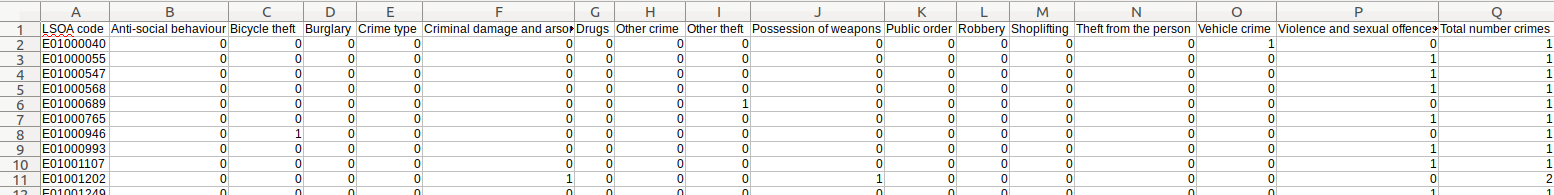
\includegraphics[width=1\textwidth]{images/csv_street_crime.png}
	\caption{$sw\_5forces\_street\_by\_lsoa.csv$}
	\label{ft_fig_firstfig3}
\end{figure}


This file contains our own geographical data regarding the number of crimes per LSOA.
Each row contains data for an LSOA. This file also contains a field with a unique code for each LSOA, which matches a field in the attribute table for the corresponding shapefile.\\

\textit{Note: QGIS has a function "point to polygon", but the third party LSOA shapefile contains errors which need addressing before this can work. Instead we do our calculations in python outside of QGIS and perform a table join.}

\section{Add delimited text layer}
Let's add this delimited text layer
\begin{tabular}{@{}c@{}}
\includegraphics[width=4ex]{images/add_delimited_text_layer_icon.png}\end{tabular}
. \\

%In QGIS, opening a csv file is known as \textit{adding a delimited textlayer}. There are many ways to add a delimited text layer:
%\begin{enumerate}[~~~1)]
%	\item
%	Menu: Layer $\rightarrow$ Add Layer $\rightarrow$ Add Delimited Text Layer
%	
%	\item 
%	\textit{Add delimited text layer} icon on a toolbar
%	\begin{tabular}{@{}c@{}}
\includegraphics[width=4ex]{images/add_delimited_text_layer_icon.png}\end{tabular}
%	
%	\item 
%	Use \textit{browse panel} to navigate to the file location
	
%	\item 
%	Data Source Manager icon
%	\begin{tabular}{@{}c@{}}
\includegraphics[width=4ex]{images/data_source_manager_icon.png}\end{tabular}
	
	
%\end{enumerate}


Within the \textit{Data Source Manager / Delimited text} window, choose these settings:\\
\textbf{File name:} Navigate to the csv file: $sw\_5forces\_street\_by\_lsoa.csv$\\
\textbf{Layer name} (what appears in the \textit{Layers Panel}, so choose something meaningful): street\_crime\\
\textbf{File Format}: CSV (comma separated values)\\
\textbf{Geometry Definition}: No geometry\\
\textbf{Geometry CRS}: EPSG4326 – WGS 84 (leave as default)\\
(Note: The top row of the csv file is used as the field titles.)\\
\textbf{Add}.\\

\begin{figure}[!h]
      	\centering
      	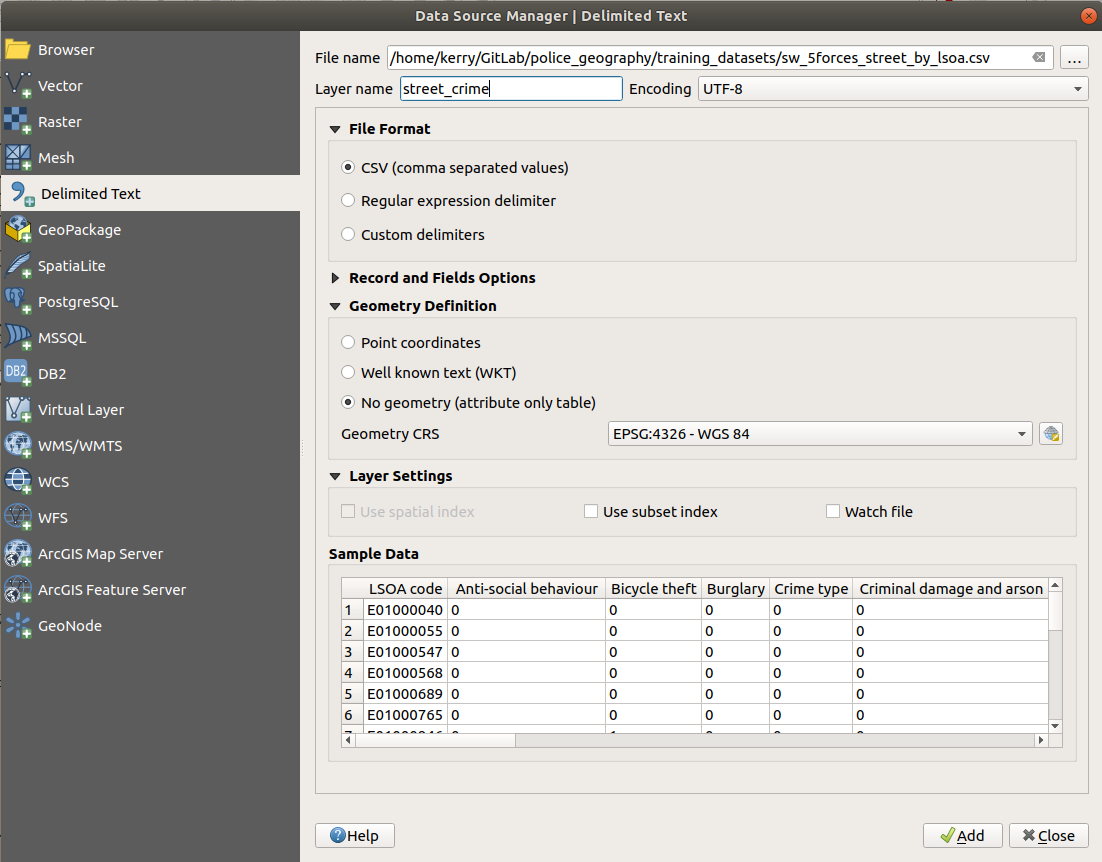
\includegraphics[width=1\textwidth]{images/data_source_manager_window_delimited_text.png}
      	\caption{Adding the delimited text file $sw\_5forces\_street\_by\_lsoa.csv$}
      	\label{ft_fig_firstfig3}
\end{figure}
        
The file will appear in the list in the \textit{Layers Panel} – but will not appear on the map canvas yet as it does not contain geometry data.
Need to join this data to the LSOA shapefile.

\null\newpage

\section{Table join: Join data from csv file to shapefile}
To join our geographical data to the shapefile layer, open layer properties for the shapefile layer: Right click $\rightarrow$ Properties, or double click on the layer name in the \textit{Layers panel}.\\

Firstly, select \textit{Source Fields} on the LHS pane. See there's only 4 fields in the original \textit{Attribute Table}.\\

Select \textbf{Join} in the LHS pane.\\
To initiate a new join select 
\begin{tabular}{@{}c@{}}
\includegraphics[width=4ex]{images/green_button_icon.png}\end{tabular}
at bottom\\
\textbf{Join layer} = csv filename\\
\textbf{Join field} = field name in the csv file that contains the common codes\\
\textbf{Target field} = field name in the shapefile that contains the common codes\\

(Can check which fields we want to use by opening both attribute tables \textit{attribute tables}, for LSOA shapefile, and for street\_crime).

\begin{figure}[!h]
	\centering
	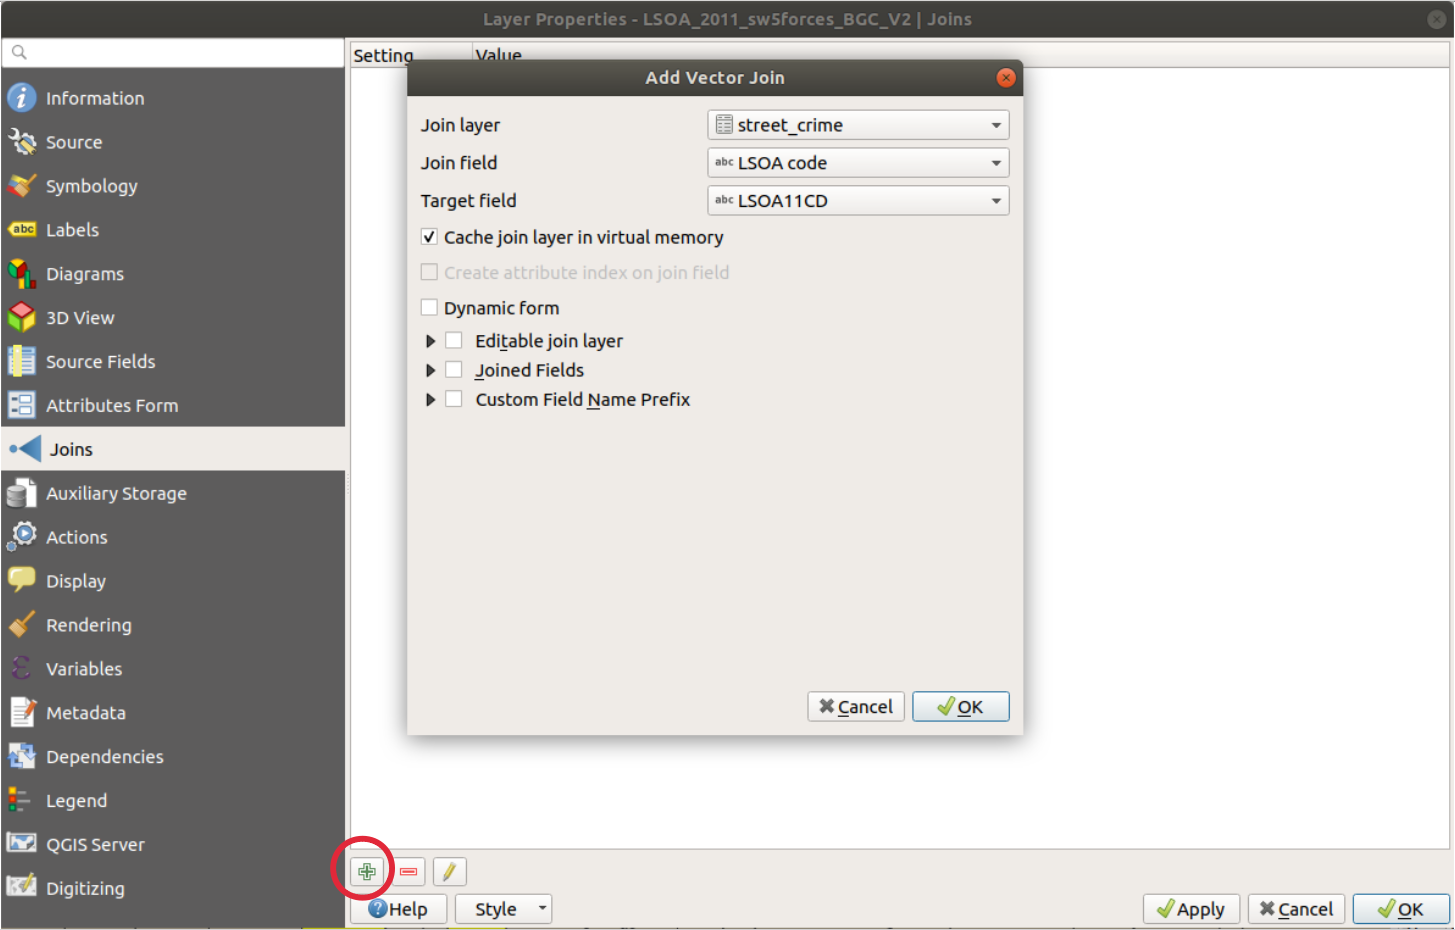
\includegraphics[width=0.8\textwidth]{images/layer_properties_join.png}
	\caption{Joining the csv data to the shapefile based on a common unique field value}
	\label{ft_fig_firstfig3}
\end{figure}

\textbf{Apply}\\

Select \textit{Source Fields} on LHS pane. This shows that new fields have been added to the attribute of the shapefile layer. Can also see this in the shapefile’s \textit{attribute table}. 

\null\newpage

\begin{figure}[!h]
	\centering
	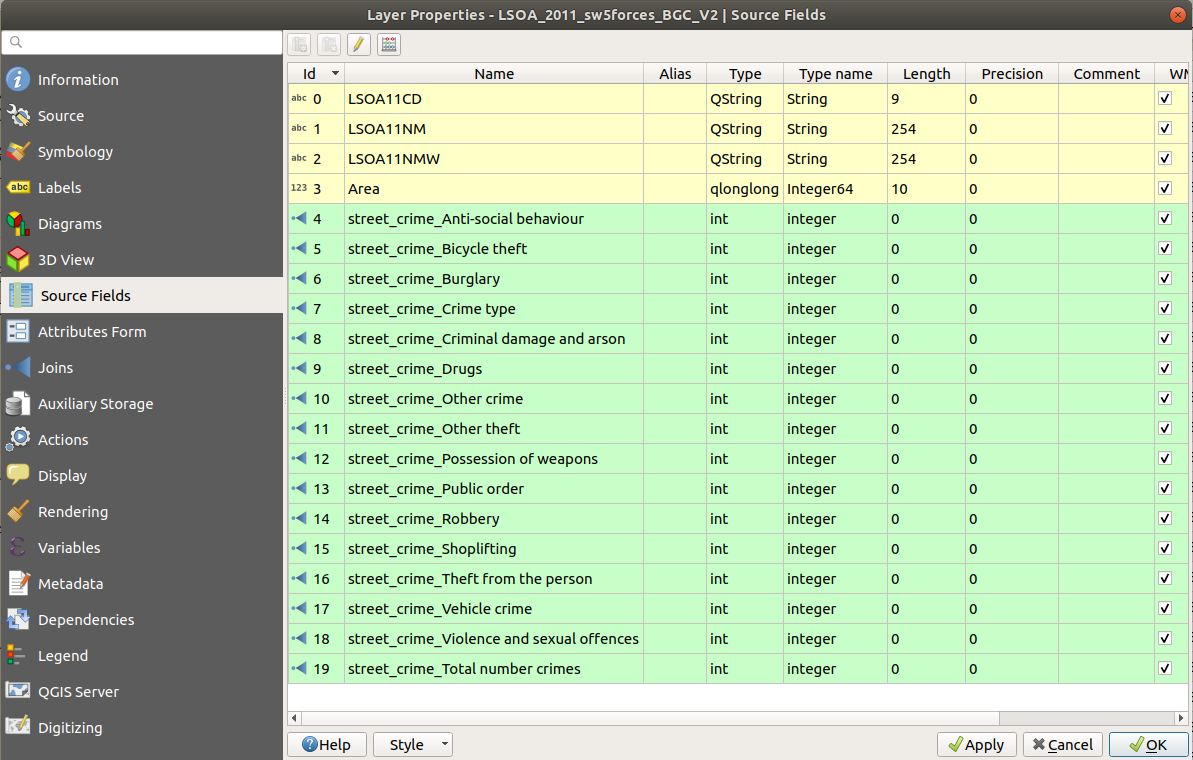
\includegraphics[width=0.8\textwidth]{images/layer_properties_source_fields.png}
	\caption{Source fields showing the original shapefile fields (yellow) and joined fields (green)}
	\label{ft_fig_firstfig3}
\end{figure}

Click OK.\\
\\
Nothing has changed in the map canvas yet. We need to add symbology to the shapefile layer.